\documentclass[conference]{IEEEtran}
\usepackage{times}
\usepackage[numbers]{natbib}
\usepackage{graphicx}
\usepackage{booktabs}
\usepackage{amsmath}
\usepackage{algorithm}
\usepackage{algpseudocode}
\usepackage[bookmarks=true]{hyperref}

\pdfinfo{
   /Author (Zhijie Chen and Shiyi Xiao)
   /Title  (Dynamic-Obstacle Parkour with Quadruped Robots)
   /CreationDate (D:20260530120000)
   /Subject (Intelligent Robot Midterm Report)
   /Keywords (quadruped parkour; reinforcement learning; imitation learning; dynamic obstacles)
}

\begin{document}

\title{Dynamic-Obstacle Parkour with Quadruped Robots}

\author{
   \IEEEauthorblockN{Zhijie Chen}
   \IEEEauthorblockA{Shanghai Jiao Tong University}
   \and
   \IEEEauthorblockN{Shiyi Xiao}
   \IEEEauthorblockA{Shanghai Jiao Tong University}
}

\maketitle

\begin{abstract}
   We present midterm progress on a research project on quadruped parkour that builds on \emph{Extreme Parkour with Legged Robots}~\citep{cheng2023parkour}. Our updated goal is to extend the original static-obstacle simulation benchmark toward dynamic parkour, where obstacle positions, support surfaces, and target waypoints change during execution. Since all current experiments are in Isaac Gym and time is limited, we drop the robust-depth-perception branch proposed earlier and focus on infrastructure and training stability for dynamic obstacles. We have implemented a dynamic A1 parkour task with scripted obstacle actors, a unified terrain-parameter interface, a video recorder for rollout inspection, and a DAgger-style imitation pretraining stage before reinforcement-learning fine-tuning. Preliminary results show that the original base pipeline reaches about $0.996$ waypoints on static terrain but only $0.399$ on dynamic terrain, while imitation-pretrained dynamic fine-tuning improves the best observed dynamic result to about $0.704$ waypoints.
\end{abstract}

\IEEEpeerreviewmaketitle

\section{Introduction}
Legged parkour requires contact-rich control, rapid perception-action coupling, and robust timing around terrain discontinuities. \citet{cheng2023parkour} demonstrated that a Unitree A1 robot can traverse hurdles, gaps, ramps, and steps by training a privileged base policy in simulation and distilling it to a deployable depth-based policy. This provides a strong baseline, but the original task primarily uses static geometry.

Our project asks how far this framework can be pushed when obstacles become dynamic. Compared with static parkour, dynamic-obstacle parkour requires the controller to react not only to terrain shape but also to time-varying obstacle state. This midterm report therefore emphasizes the infrastructure needed to study that question: dynamic terrain generation, scripted obstacle actors, rollout visualization, and a new imitation pretraining stage. We intentionally narrow the proposal by dropping the robust-depth-perception branch. Because the current platform is simulator-only, improvements from depth augmentation or temporal fusion would be hard to validate against real sensing artifacts within the remaining course schedule.

\section{Related Work}
Recent legged-locomotion systems combine reinforcement learning, privileged training signals, and onboard sensing to traverse challenging terrain~\citep{kumar2021rma,agarwal2022legged,miki2022learning}. The baseline of \citet{cheng2023parkour} is closest to our project: it trains a privileged parkour policy and then distills it to depth input. We retain this staged structure and modify the environment and training initialization rather than designing a new controller from scratch.

Our imitation pretraining stage follows the motivation of DAgger~\citep{ross2011dagger}: policies trained only on expert-state distributions can fail after their own early mistakes, so the learner should also train on states induced by its current behavior. We use this idea before PPO-style base fine-tuning~\citep{schulman2017ppo}. The simulator implementation uses Isaac Gym~\citep{makoviychuk2021isaacgym}, allowing many parallel dynamic parkour environments on GPU.

\section{Technical Approach}
Figure~\ref{fig:pipeline} summarizes the current pipeline. We first reproduce the original static-terrain base and distillation stages. We then train on the new \texttt{a1\_dynamic} task, which inherits the original A1 parkour configuration but replaces the terrain distribution with dynamic obstacle families. Finally, we add imitation pretraining between the static expert and dynamic base training.

The improved pipeline will augment the latent environment information with dynamic obstacle state, such as current hurdle position, gap configuration, step height, or ramp angle. In the distillation stage, the depth-based policy will be trained to recover these quantities explicitly or implicitly from observations. We will decide empirically whether ROA-style latent estimation, teacher-student distillation, or a hybrid version works better for this extension, based on both performance and training stability.

\begin{figure}[t]
   \centering
   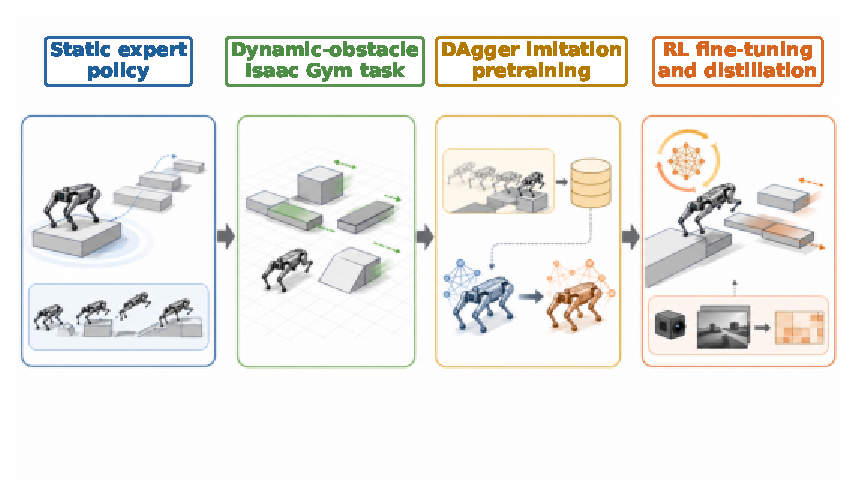
\includegraphics[width=\linewidth,trim=0 2cm 0 0,clip]{figures/pipeline_diagram.pdf}
   \caption{Current training pipeline. A static-terrain expert initializes dynamic-obstacle learning through DAgger imitation pretraining, after which the policy is fine-tuned by the original base RL stage and later prepared for camera distillation.}
   \label{fig:pipeline}
\end{figure}

\subsection{Dynamic Parkour Infrastructure}
The new task \texttt{a1\_dynamic} is registered separately from the original \texttt{a1} task. Its terrain configuration exposes a single dynamic-obstacle interface for obstacle counts, dimensions, amplitudes, periods, spacing, and difficulty-interpolated ranges. The implemented families include moving hurdles, moving gap platforms, tilting pads, moving steps, and a mixed dynamic-demo track. Terrain generation stores per-tile dynamic metadata, including obstacle pose specifications, motion groups, goal groups, and terrain difficulty.

At runtime, dynamic obstacles are Isaac Gym box actors with gravity disabled. The environment updates their root states before physics steps using scripted sinusoidal translations or rotations. Hurdles and gap platforms translate along the forward axis, steps move vertically, and tilted pads rotate about roll. Height sampling is extended so the privileged terrain observation includes both static height-field samples and the current top surfaces of dynamic actors. Dynamic waypoints are also updated when a goal is tied to a moving obstacle, so the policy is trained against the current traversable target.

We also implemented a rollout video recorder in \texttt{play.py}. It records one MP4 per environment and supports two camera modes: a yaw-following mode that tracks heading without inheriting roll or pitch, and an attached mode that follows the robot body transform. This has been useful for diagnosing dynamic-obstacle failures such as late takeoff, unstable landings, and poor timing around moving support surfaces.

\subsection{DAgger Imitation Pretraining}
Dynamic parkour is substantially harder to learn from scratch, so we added a pretraining stage that uses a static-terrain A1 base policy as an expert. The student policy is trained in the dynamic environment before normal RL fine-tuning. Expert action labels are computed with history encoding enabled, matching the inference path used by evaluation and play scripts. The student actor is optimized in both privileged and history-encoding modes, and the estimator is trained against privileged-state targets so that later fine-tuning resumes through the original training path.

\begin{algorithm}[t]
   \small
   \caption{DAgger-style imitation pretraining}
   \label{alg:dagger}
   \begin{algorithmic}[1]
      \Require static expert $\pi_E$, dynamic environment, student $\pi_\theta$
      \State Initialize teacher replay $B_E$ and student replay $B_S$
      \For{$k=0,\ldots,K-1$}
      \If{$k$ is in BC warmup}
      \State Collect observations driven by $\pi_E$
      \State Store $(o,\pi_E(o))$ in $B_E$
      \Else
      \State Collect expert-driven samples into $B_E$
      \State Collect student-driven samples into $B_S$, labeled by $\pi_E$
      \EndIf
      \State Sample balanced minibatches from $B_E$ and $B_S$
      \State Minimize $L_{\mathrm{act}}+L_{\mathrm{hist}}+L_{\mathrm{est}}$ by gradient descent
      \State Save imitation checkpoints at the normal runner interval
      \EndFor
      \State \Return $\pi_\theta$ for dynamic base RL fine-tuning
   \end{algorithmic}
\end{algorithm}

\section{Preliminary Experiments and Results}
We compare runs from the original static terrain, the original pipeline applied to dynamic terrain, and the new imitation-pretrained dynamic pipeline. The reported metric is the mean number of waypoints reached during evaluation, where higher values indicate better parkour progress through the track. Training curves are shown in Figure~\ref{fig:curves}, and the best observed checkpoint values are summarized in Table~\ref{tab:results}.

\begin{figure}[t]
   \centering
   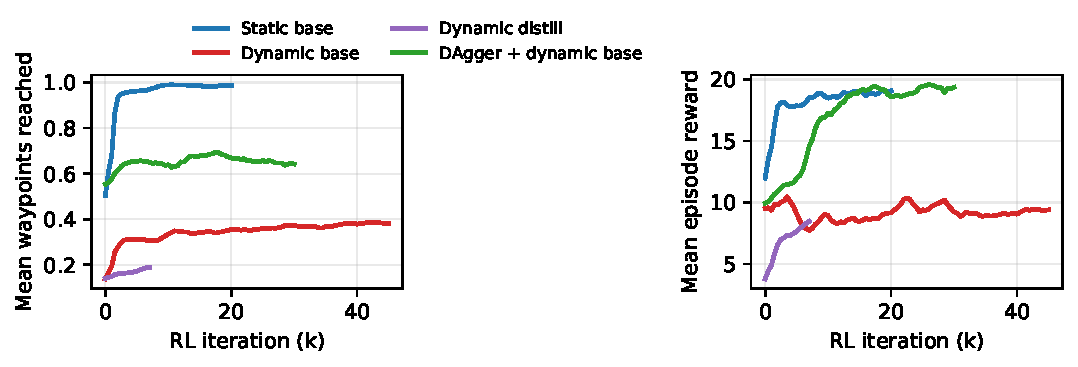
\includegraphics[width=\linewidth]{figures/training_curves.pdf}
   \caption{Smoothed preliminary evaluation curves. The original base pipeline transfers poorly from static to dynamic terrain, while DAgger imitation pretraining gives a better starting point for dynamic RL fine-tuning.}
   \label{fig:curves}
\end{figure}

\begin{table}[t]
   \centering
   \caption{Best observed preliminary results from available logs. Distillation on dynamic terrain is still incomplete.}
   \label{tab:results}
   \begin{tabular}{lccc}
      \toprule
      Run                   & Checkpoint & Waypoints & Reward \\
      \midrule
      Static base           & 9500       & 0.996     & 18.73  \\
      Static distill        & 10000      & 0.936     & 18.26  \\
      Dynamic base          & 38500      & 0.399     & 9.33   \\
      Dynamic distill       & 7000       & 0.192     & 8.51   \\
      DAgger + dynamic base & 17500      & 0.704     & 19.35  \\
      \bottomrule
   \end{tabular}
\end{table}

These results support two observations. First, the reproduced static-terrain pipeline behaves as expected, reaching nearly one waypoint on average in the available evaluation logs. Second, directly applying the original base-training pipeline to dynamic terrain is much less effective, plateauing around $0.4$ waypoints despite a longer run. The imitation-pretrained dynamic run reaches about $0.704$ waypoints, suggesting that a static expert can provide useful initialization even under distribution shift. The dynamic distillation stage is not yet a fair final comparison because that run has not completed.

\section{Remaining Plan}
The next step is to finish longer dynamic base and distillation runs, then evaluate policies by dynamic obstacle family rather than only by aggregate waypoint count. We will also use the video recorder to categorize failure modes, especially mistimed takeoff, obstacle collision, and unstable landing. If time permits, we will add a small ablation comparing DAgger pretraining against direct static-policy initialization and offline behavior cloning. The final report will focus on whether imitation pretraining consistently improves dynamic parkour learning and on which obstacle families remain bottlenecks.

\bibliographystyle{plainnat}
\bibliography{references}

\end{document}
